\begin{adjustbox}{width=\textwidth}
	\begin{tikzpicture}[every node/.style={inner sep=0,outer sep=0}]
	
		\node [anchor=north east] (img1) at (-0.05\textwidth,0) {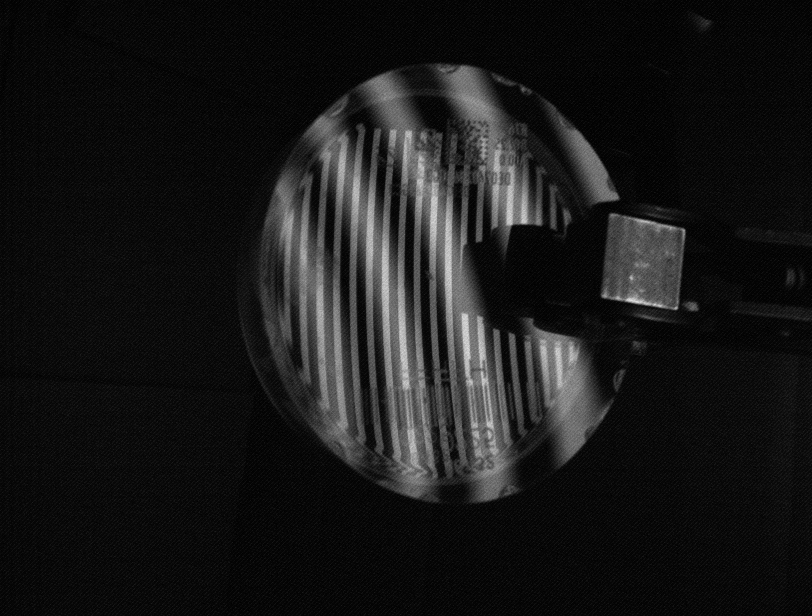
\includegraphics[width=.45\textwidth]{05_ergebnisse/ergDiskussion/figures/impulsBeleuchtung_RR}};
		\node [below=0.2cm of img1, align=center] {Aufnahme des Streifenmusters \\ mit Rückseitenreflex};
		\node [anchor=north west] (img2) at (0.05\textwidth,0) {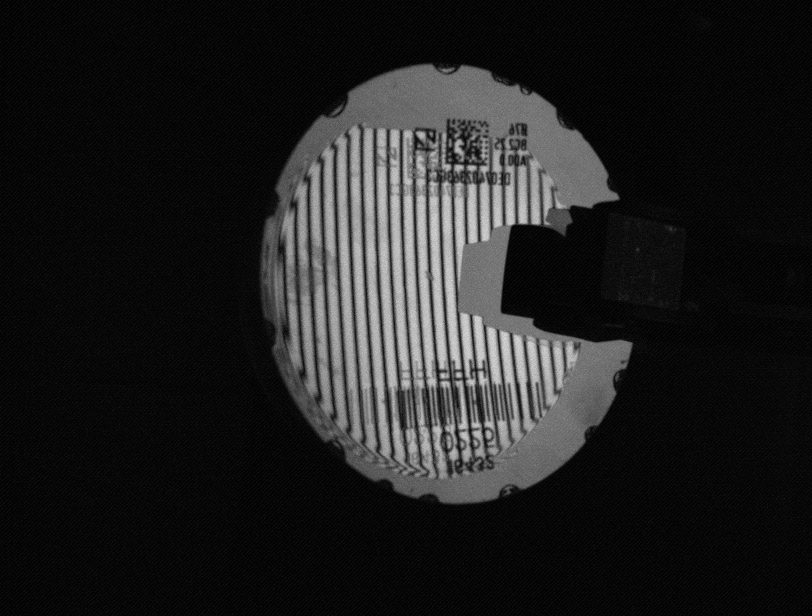
\includegraphics[width=.45\textwidth]{05_ergebnisse/ergDiskussion/figures/combine_RR}};
		\node [below=0.2cm of img2, align=center] {Ergebnisbild des Verfahren \\ Sichtprüfung durch Lichtstreuung};
		
		\draw[very thick,-{Latex[width=3mm]},shorten >=0.02\textwidth,shorten <=0.02\textwidth] (img1.east) -- (img2.west);
		
	\end{tikzpicture}
\end{adjustbox}
\caption[Rückseitenreflex bei \glqq Sichtprüfung durch Lichtstreuung\grqq]{Auswirkungen des Rückseitenreflexes bei \glqq Sichtprüfung durch Lichtstreuung\grqq. Es entstehen vertikale Streifen auf der Rückseite des Brillenglases.}